\documentclass[a4paper, 11pt]{article}
\usepackage{float}
%\usepackage[UTF8]{ctex}
%\usepackage{fontspec}
%\setmainfont{Fira Code}	% 设置全局英文字体(代码)
%\setCJKmainfont{宋体} 	% 设置全局中文字体

%\usepackage{fancyhdr} 	% 页眉页脚
%\usepackage{lastpage} 	% 获得总页数

% 插入图片的宏包
\usepackage{subfigure}
\usepackage{graphicx} 	% 插入图片的宏包
\graphicspath{{pic/}} 	% 在于.tex同级的目录下创建名为pic的文件夹,存放图片

% 超链接
\usepackage[colorlinks,linkcolor=red]{hyperref}

% 防止右边界越界(取消首段缩进?)
\raggedright 		  
% 首行缩进两格
\usepackage{indentfirst}
\setlength{\parindent}{2em}
% 页边距
\usepackage{geometry}
\geometry{a4paper,left=3cm,right=3cm,top=2cm,bottom=2cm}

\usepackage{amssymb} 	%不等号 等符号
\usepackage{amsmath} 	% 这是用于数学公式编辑的宏包
\usepackage{listings} 	% 用于插入代码块的宏包
\usepackage{xcolor}
\usepackage{color}
\usepackage{longtable}

\title{	
\normalfont \normalsize
\textsc{School of Data and Computer Science, Sun Yat-sen University} \\ [25pt] %textsc small capital letters
\rule{\textwidth}{0.5pt} \\[0.4cm] % Thin top horizontal rule
\huge Chinese Segmentation Using BiLSTM-CRF \\ % The assignment title
\rule{\textwidth}{2pt} \\[0.5cm] % Thick bottom horizontal rule
\author{18308045 Zhengyang Gu}
\date{\normalsize\today}
}

\begin{document}
\maketitle
\tableofcontents
\newpage
\definecolor{mygreen}{rgb}{0,0.6,0}
\definecolor{mygray}{rgb}{0.5,0.5,0.5}
\definecolor{mymauve}{rgb}{0.58,0,0.82}
% 定义一些自用的颜色深度
% 设置显示代码颜色
\lstset{
      backgroundcolor=\color{white},  % 代码块背景颜色
      %basicstyle=\footnotesize \fontspec{Fira Code},       % 用于代码的前端显示
      breakatwhitespace=false,        % 若设置中断则发现在空白区
      breaklines=true,                % 设置自动断行
      captionpos=bl,                  % 设置标题位置为底端显示
      commentstyle=\color{mygreen},   % 注释风格颜色
      deletekeywords={...},           % 用于删除某关键字
      escapeinside={\%*}{*)},
      extendedchars=true,
      frame=single,                   % 在代码块区域增加边框
      keepspaces=true,
      keywordstyle=\color{blue},      % 关键词的颜色
      language=python,               	% 要在代码块插入的代码类型
      morekeywords={*,...},           % if you want to add more keywords to the set
      numbers=left,
      numbersep=5pt,
      numberstyle=\tiny\color{mygray},% 行号字体的颜色
      rulecolor=\color{black},
      showspaces=false,
      showstringspaces=false,
      showtabs=false,
      stepnumber=1,                   % the step between two line-numbers
      stringstyle=\color{red},        % 双引号内的颜色
      tabsize=2,
}
\section{README!!!}
My vscode crashed when I was editing the tex file causing my losing the tex file, but the pdf of the first part is retained.
Therefore, I splited the whole report into two parts.

\href{run:first_part.pdf}{The first part of the report.}

\href{https://github.com/guzy0324/BiLSTM_CRF.git}{Codes and README.md are open-sourced on github.}

\section{My Implementation}
\subsection{Tagging Using CRF}
\subsection{Training}
We can address this issue by making a few changes. Let $smat(Y_j,Y_{j+1})$ be $\alpha(Y_j)+f(X_j,Y_j)+t(Y_j,Y_{j+1})$.
$$\begin{aligned}
    \alpha(Y_{j+1})=&\log(\sum_{Y_j}\exp(\alpha(Y_j)+f(X_j,Y_j)+t(Y_j,Y_{j+1})))\\
    =&\log(\sum_{Y_j}\exp(smat(Y_j,Y_{j+1})))\\
    =&\log(\sum_{Y_j}\exp(smat(Y_j,Y_{j+1})-\max_{Y_j}smat(Y_j,Y_{j+1})))+\max_{Y_j}smat(Y_j,Y_{j+1})
\end{aligned}$$
Then when after we calculate the \textbf{exp}, the max number we get is $1$, so there won't be any overflow errors in python.
In addition, I add the batch to the first dimension. The implementation of the \textbf{log\_sum\_exp} is as follows.
\begin{lstlisting}
def log_sum_exp(smat_batch):
   vmax_batch = smat_batch.max(dim=1, keepdim=True).values
   return (smat_batch - vmax_batch).exp().sum(axis=1, keepdim=True).log() + vmax_batch
\end{lstlisting}

\subsection{Estimating The $f(X_i,Y_i)$ Using BiLSTM}
I use the BiLSTM implemented in pytorch, so there isn't much to say in this section.

\subsection{Batch}
I add the batch to the first dimension, so I have to make the \textbf{batch\_first} to be \textbf{True}.
\begin{lstlisting}
self.lstm = nn.LSTM(embedding_dim, hidden_dim // 2, num_layers=1, bidirectional=True, batch_first = True)
\end{lstlisting}
However, the \textbf{batch\_first} only affects the input and output but not the hidden state, so when initializing the hidden state I have
to add the batch to the second dimension.
\begin{lstlisting}
hidden_batch = torch.randn(2, self.batch_size, self.hidden_dim // 2).to(self.device),\
        torch.randn(2, self.batch_size, self.hidden_dim // 2).to(self.device)
\end{lstlisting}
In addition, the loss of a batch here is defined as the average value of each \textbf{neg\_log\_likelihood} in the batch.
\begin{lstlisting}
return (forward_score_batch - gold_score_batch).sum(0) / self.batch_size
\end{lstlisting}

\subsection{Hyperparameters}
\begin{itemize}
\item GPU: If \textbf{True}, GPU will be used to improve the speed of training.
\item LR: Learning rate of the optimizer.
\item MAX\_EPOCH: The max number of epoches when training.
\item BATCH\_SIZE: The size of each batch.
\item EMBEDDING\_DIM: The dimension of the word embedding.
\item HIDDEN\_DIM: The dimension of BiLSTM' s hidden state.
\item SHUFFLE: If \textbf{True}, every epoch the training data will be shuffled.
\end{itemize}

\section{Result}
\subsection{Hyperparameters}
I tested different values of some of the hyperparameters ahead of the learning process to choose a fairly good combination of
hyperparameters.
\begin{table}[ht]
\begin{tabular}{llllll}
MAX\_EPOCH & BATCH\_SIZE & EMBEDDING\_DIM & HIDDEN\_DIM & Time  & F1                 \\
1          & 128         & 16             & 16          & 17:04 & 0.789882198385716  \\
1          & 128         & 128            & 16          & 17:47 & 0.7985092541747879 \\
1          & 128         & 128            & 128         & 17:35 & 0.8670882556323042 \\
1          & 256         & 128            & 128         & 19:34 & 0.8519033872880736
\end{tabular}
\end{table}

\subsection{Final Result}
The hyperparameters I choose are shown as below.
\begin{lstlisting}
GPU = True
LR = 0.01
MAX_EPOCH = 128
BATCH_SIZE = 128
EMBEDDING_DIM = 128
HIDDEN_DIM = 128
SHUFFLE = True
\end{lstlisting}

Here came an error when I was training the model.
\begin{figure}[H]
      \centering
      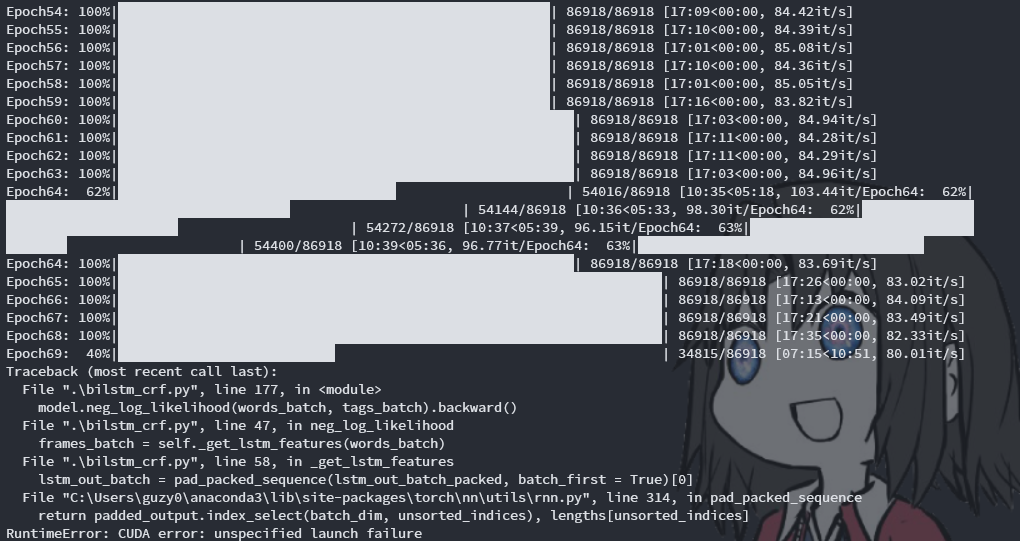
\includegraphics[width = 0.8 \textwidth]{error.png}
      \caption{Error I met}
\end{figure}
Hence, I just trained the model for 69 epoches. The bug is just related to the CUDA configuration, but has nothing to do with my codes.
\cite{ref1}

The average F1 score tested on the \textbf{msr\_test\_gold.utf8} is shown as below.
\begin{figure}[H]
      \centering
      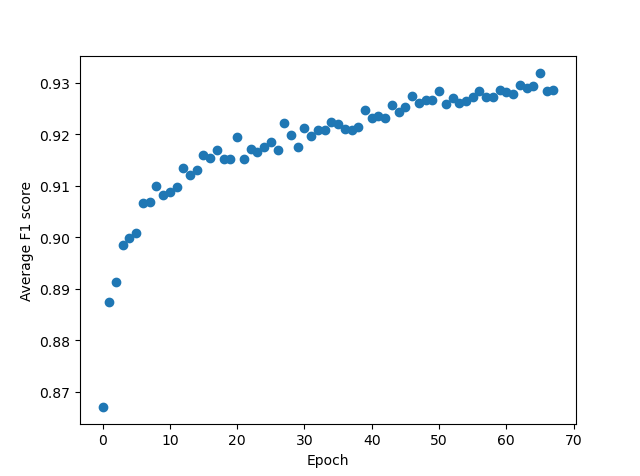
\includegraphics[width = 0.8 \textwidth]{Figure_1.png}
      \caption{Average F1 score}
\end{figure}
We can find that the F1 score is still increasing.

The segmentation result of \textbf{msr\_test.utf8} is \href{result.utf8}{result.utf8}.

\section{Conclusions And Bonuses I May Get}
\begin{enumerate}
      \item I implemented the BiLSTM-CRF model to accomplish the Chinese segmentation task.
      \item I use batch and GPU to speed up the training process.
      \item I tested different combination of hyperparameters ahead of training.
      \item I compose my report in English, although it may be not fluent.
\end{enumerate}

Future work may include the experiment with more running epochs.

\begin{thebibliography}{99}
    \bibitem{ref1} \url{https://www.cnblogs.com/dgwblog/p/12868068.html}

\end{thebibliography}




\end{document}





